% ============================================================================
% Discussion
% ============================================================================
\section{Discussion}
\label{sec:discussion}

The main goal of this project was to reproduce the paper by  Litwin-Kumar and Doiron (2012) \textcolor{red}{(add reference)}. Through replicating their results, we got our first experience in building a computational experimental model while working as a team. We acquired the key skills in doing neural network simulations using Brian2 and in converting the technical descriptions found in the original paper into actual code. In this process we also had to convert some key equations to a format more applicable to the Brian2 framework, since the paper Litwin-Kumar and Doiron (2012) \textcolor{red}{(add reference)} did not use Python.

To understand how successful our replication of the original paper was, Figure~\ref{fig:our_results} and Figure~\ref{fig:original_results} give us a comprehensive comparison between our work and the paper.

\begin{figure}[!htbp]
    \centering
    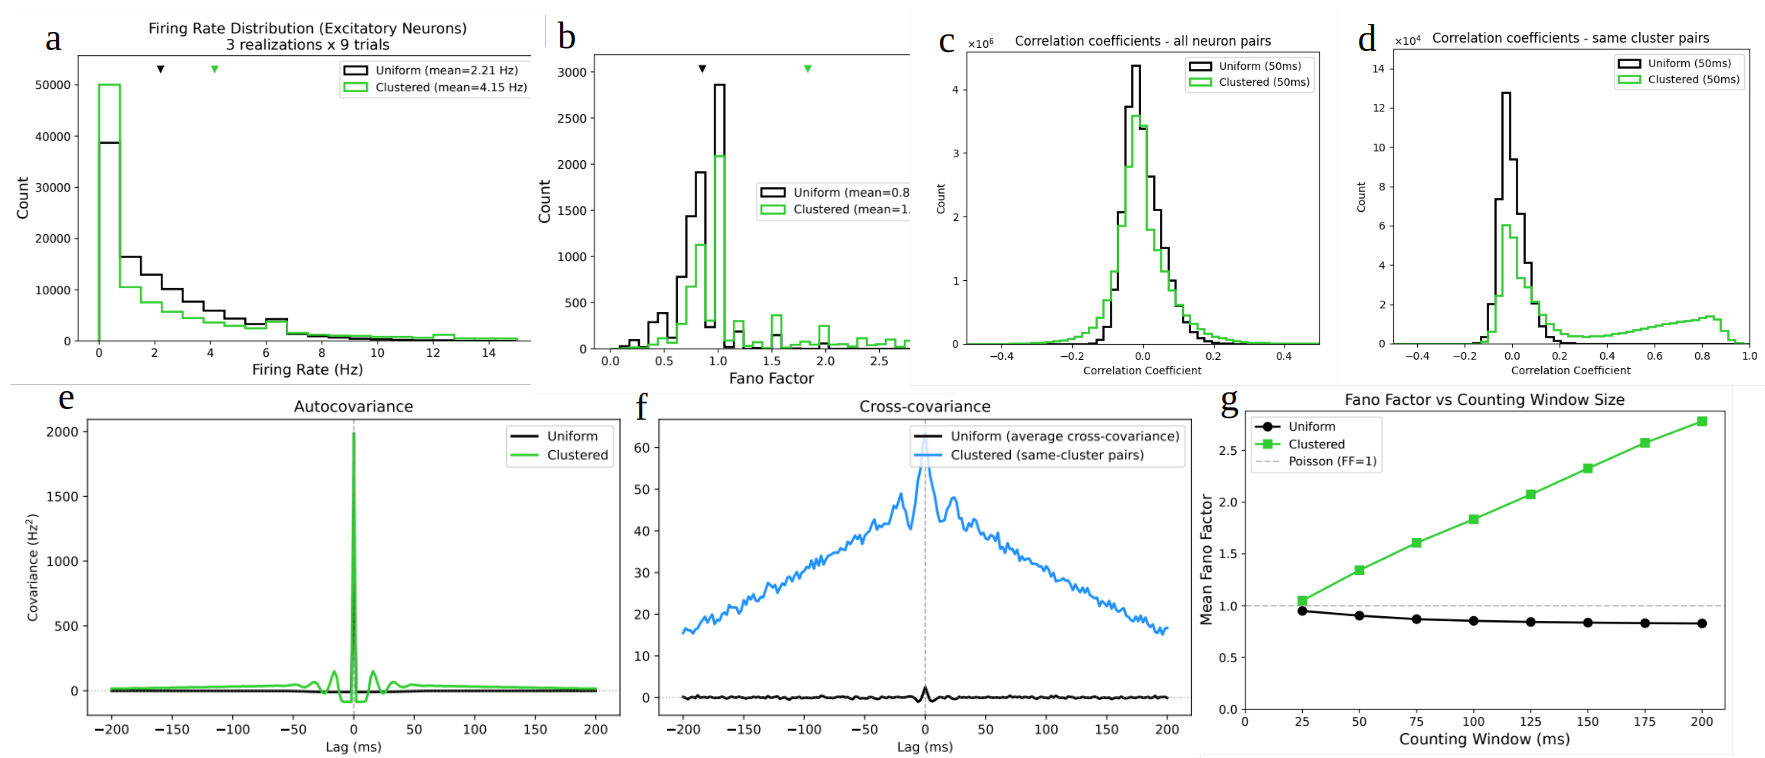
\includegraphics[width=\columnwidth]{report/figures/our_results.png}
    \caption{The graphs combined together from our statistical analysis.}
    \label{fig:our_results}
\end{figure}

\begin{figure}[!htbp]
    \centering
    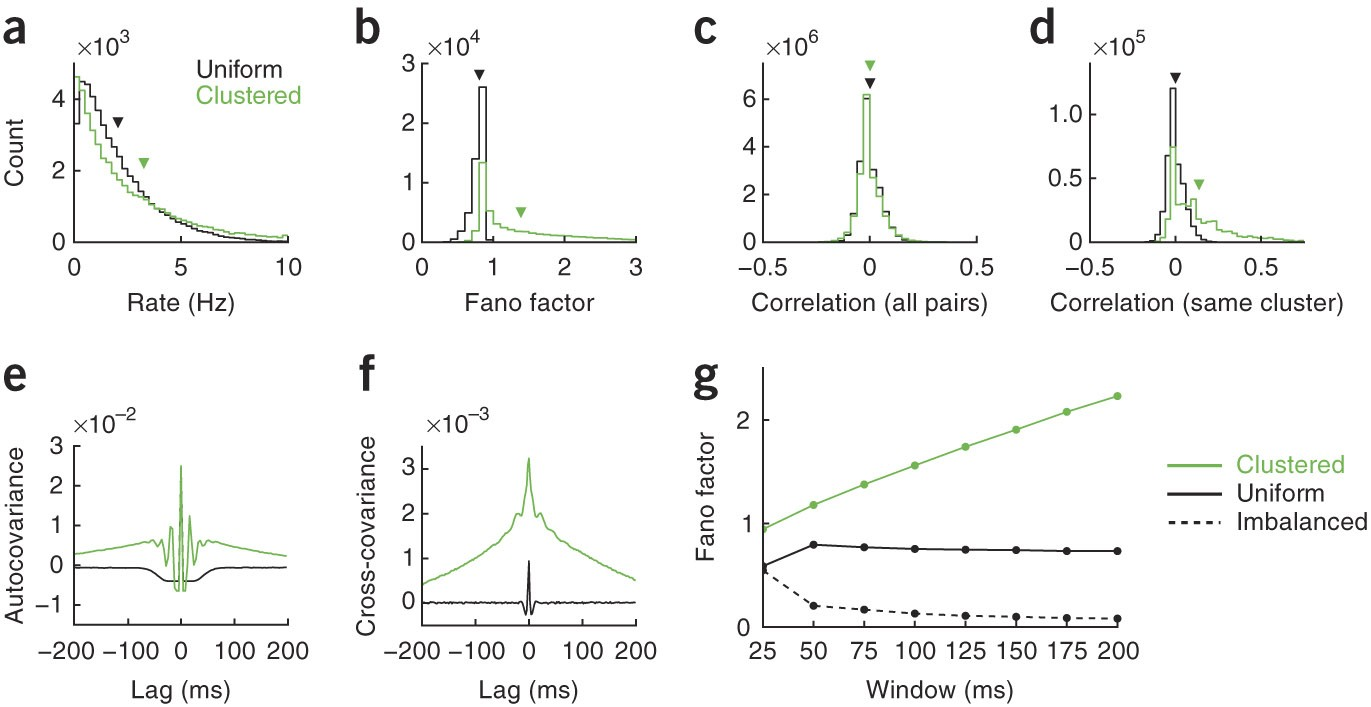
\includegraphics[width=\columnwidth]{report/figures/original_results.jpg}
    \caption{Statistical analysis results from the original paper \textcolor{red}{(add reference).}}
    \label{fig:original_results}
\end{figure}

From this comparison, we see that most of the statistical analyses are very similar. The most fundamental difference is between Figure~\ref{fig:our_results} \textbf{(d)} and Figure~\ref{fig:original_results} \textbf{(d)}. From our experiment, the correlation coefficient figure displays a long heavy tail, with a significant bump around the 0.8 mark, while the original paper displayed a gradually diminishing positive tail, having almost no coefficients at 0.8.

While it is hard to know exactly the firing dynamics of the network in the original paper, we can still make a guess at the possible ex